%%%%%%%% ICML 2026 Workshop on AI Forecasting submission %%%%%%%%
\documentclass{article}

\usepackage{microtype}
\usepackage{graphicx}
\usepackage{subcaption}
\usepackage{booktabs}
\usepackage{hyperref}
\newcommand{\theHalgorithm}{\arabic{algorithm}}

\usepackage{icml2026}

\usepackage{amsmath}
\usepackage{amssymb}
\usepackage{mathtools}
\usepackage{amsthm}
\usepackage[capitalize,noabbrev]{cleveref}

\usepackage{tikz}
\usepackage{pgfplots}
\pgfplotsset{compat=1.18}
\usetikzlibrary{positioning}
\usepgfplotslibrary{statistics}

\pgfplotsset{
  every axis/.append style={
    font=\footnotesize,
    label style={font=\footnotesize},
    tick label style={font=\scriptsize},
    legend style={font=\scriptsize, draw=none, fill=none, inner sep=1pt},
    legend cell align=left,
  },
  reasoning/.style={color=blue!70!black, mark options={fill=blue!70!black}},
  nonreasoning/.style={color=orange!85!black, dashed, mark options={fill=orange!85!black, solid}},
  reasoningmark/.style={color=blue!70!black, mark=*, mark size=2pt},
  nonreasoningmark/.style={color=orange!85!black, mark=square*, mark size=2pt},
}

% Auto-generated by code/emit_data_tex.py — DO NOT EDIT BY HAND.
% Re-run `python code/emit_data_tex.py` after `python run.py`.
\def\dosesAggLZero{0.521}
\def\dosesAggSELZero{0.019}
\def\dosesAggLOne{0.523}
\def\dosesAggSELOne{0.017}
\def\dosesAggLTwo{0.654}
\def\dosesAggSELTwo{0.015}
\def\dosesAggLThree{0.687}
\def\dosesAggSELThree{0.015}
\def\dosesRefLZero{0.521}
\def\dosesRefLOne{0.681}
\def\dosesRefLTwo{0.840}
\def\dosesRefLThree{1.000}
\def\dosesAggCoords{(0,0.521) (1,0.523) (2,0.654) (3,0.687)}
\def\dosesRefCoords{(0,0.521) (1,0.681) (2,0.840) (3,1.000)}
\def\perModelPlots{\addplot+[reasoning,mark=*,thick] coordinates {(0,0.502) (1,0.540) (2,0.685) (3,0.720)};\addlegendentry{GPT-5 mini (R)}
\addplot+[nonreasoning,mark=*,thick] coordinates {(0,0.533) (1,0.539) (2,0.668) (3,0.709)};\addlegendentry{GPT-4o}
\addplot+[reasoning,mark=*,thick] coordinates {(0,0.510) (1,0.506) (2,0.626) (3,0.664)};\addlegendentry{Opus 4.7 (R)}
\addplot+[nonreasoning,mark=*,thick] coordinates {(0,0.523) (1,0.494) (2,0.620) (3,0.684)};\addlegendentry{Sonnet 4.6}
\addplot+[nonreasoning,mark=*,thick] coordinates {(0,0.577) (1,0.552) (2,0.694) (3,0.702)};\addlegendentry{Haiku 4.5}
\addplot+[reasoning,mark=*,thick] coordinates {(0,0.500) (1,0.508) (2,0.660) (3,0.679)};\addlegendentry{GPT-5 (R)}
\addplot+[reasoning,mark=*,thick] coordinates {(0,0.507) (1,0.521) (2,0.624) (3,0.650)};\addlegendentry{o3 (R)}}
\def\slopeBrierPlots{\addplot+[only marks,reasoningmark] coordinates {(0.080,0.139)};
\node[font=\tiny] at (axis cs:0.080,0.139) [anchor=south west,xshift=2pt,yshift=2pt] {GPT-5 mini};
\addplot+[only marks,nonreasoningmark] coordinates {(0.066,0.141)};
\node[font=\tiny] at (axis cs:0.066,0.141) [anchor=south west,xshift=2pt,yshift=2pt] {GPT-4o};
\addplot+[only marks,reasoningmark] coordinates {(0.058,0.197)};
\node[font=\tiny] at (axis cs:0.058,0.197) [anchor=south west,xshift=2pt,yshift=2pt] {Opus 4.7};
\addplot+[only marks,nonreasoningmark] coordinates {(0.079,0.186)};
\node[font=\tiny] at (axis cs:0.079,0.186) [anchor=south west,xshift=2pt,yshift=2pt] {Sonnet 4.6};
\addplot+[only marks,nonreasoningmark] coordinates {(0.049,0.141)};
\node[font=\tiny] at (axis cs:0.049,0.141) [anchor=south west,xshift=2pt,yshift=2pt] {Haiku 4.5};
\addplot+[only marks,reasoningmark] coordinates {(0.069,0.170)};
\node[font=\tiny] at (axis cs:0.069,0.170) [anchor=south west,xshift=2pt,yshift=2pt] {GPT-5};
\addplot+[only marks,reasoningmark] coordinates {(0.053,0.180)};
\node[font=\tiny] at (axis cs:0.053,0.180) [anchor=south west,xshift=2pt,yshift=2pt] {o3};}
\def\slopeBoxReasoningLowerWhisker{-0.166}
\def\slopeBoxReasoningLowerQuartile{0.005}
\def\slopeBoxReasoningMedian{0.038}
\def\slopeBoxReasoningUpperQuartile{0.119}
\def\slopeBoxReasoningUpperWhisker{0.289}
\def\slopeBoxNonLowerWhisker{-0.187}
\def\slopeBoxNonLowerQuartile{0.008}
\def\slopeBoxNonMedian{0.036}
\def\slopeBoxNonUpperQuartile{0.138}
\def\slopeBoxNonUpperWhisker{0.300}
\def\nQuestions{40}
\def\nModels{7}
\def\pearsonR{-0.043}
\def\pearsonP{0.927}
\def\partialR{-0.545}
\def\brierLzeroLthreeR{0.727}
\def\brierLzeroLthreeP{0.0641}
\def\mannWhitneyP{0.704}
\def\meanSlopeReasoning{0.065}
\def\meanSlopeNonReasoning{0.064}
\def\fracQuestionVar{0.872}
\def\fracModelVar{0.008}
\def\fracQuestionVarPct{87.2}
\def\fracModelVarPct{0.8}
\def\fracRationalGain{0.346}
\def\fracRationalGainPct{34.6}
\def\perModelTableRows{GPT-5 mini & Yes & 0.333 & 0.139 & 0.080 & 0.438 \\
GPT-4o & No & 0.290 & 0.141 & 0.066 & 0.376 \\
GPT-5 & Yes & 0.355 & 0.170 & 0.069 & 0.358 \\
Sonnet 4.6 & No & 0.334 & 0.186 & 0.079 & 0.338 \\
Opus 4.7 & Yes & 0.371 & 0.197 & 0.058 & 0.315 \\
Haiku 4.5 & No & 0.244 & 0.141 & 0.049 & 0.297 \\
o3 & Yes & 0.332 & 0.180 & 0.053 & 0.291 \\}
\def\brierLoLthreePlots{\addplot+[only marks,reasoningmark] coordinates {(0.333,0.139)};
\node[font=\tiny] at (axis cs:0.333,0.139) [anchor=north west,xshift=2pt,yshift=-2pt] {GPT-5 mini};
\addplot+[only marks,nonreasoningmark] coordinates {(0.290,0.141)};
\node[font=\tiny] at (axis cs:0.290,0.141) [anchor=north west,xshift=2pt,yshift=-2pt] {GPT-4o};
\addplot+[only marks,reasoningmark] coordinates {(0.371,0.197)};
\node[font=\tiny] at (axis cs:0.371,0.197) [anchor=north west,xshift=2pt,yshift=-2pt] {Opus 4.7};
\addplot+[only marks,nonreasoningmark] coordinates {(0.334,0.186)};
\node[font=\tiny] at (axis cs:0.334,0.186) [anchor=south west,xshift=3pt,yshift=1pt] {Sonnet 4.6};
\addplot+[only marks,nonreasoningmark] coordinates {(0.244,0.141)};
\node[font=\tiny] at (axis cs:0.244,0.141) [anchor=north west,xshift=2pt,yshift=-2pt] {Haiku 4.5};
\addplot+[only marks,reasoningmark] coordinates {(0.355,0.170)};
\node[font=\tiny] at (axis cs:0.355,0.170) [anchor=north west,xshift=2pt,yshift=-2pt] {GPT-5};
\addplot+[only marks,reasoningmark] coordinates {(0.332,0.180)};
\node[font=\tiny] at (axis cs:0.332,0.180) [anchor=north east,xshift=-3pt,yshift=-1pt] {o3};}
\def\brierLoLthreeFit{(0.239,0.130) (0.376,0.187)}
\def\BootSlopeBrierMean{-0.054}
\def\BootSlopeBrierLo{-0.848}
\def\BootSlopeBrierHi{0.781}
\def\BootPriorBrierMean{0.716}
\def\BootPriorBrierLo{0.251}
\def\BootPriorBrierHi{0.978}
\def\BootPartialMean{-0.496}
\def\BootPartialLo{-1.000}
\def\BootPartialHi{0.999}
\def\reVarQuestion{0.0544}
\def\reVarModel{0.0000}
\def\reVarResidual{0.0094}
\def\reFracQuestion{0.852}
\def\reFracQuestionPct{85.2}
\def\reFracModel{0.000}
\def\reFracModelPct{0.0}
\def\contamR{-0.362}
\def\contamP{0.0219}
\def\contamEarlyBrier{0.403}
\def\contamLateBrier{0.242}
\def\contamNearly{20}
\def\contamNlate{20}
\def\manifoldCapture{0.397}
\def\manifoldCaptureLo{0.237}
\def\manifoldCaptureHi{0.572}
\def\manifoldCapturePct{39.7}
\def\manifoldNquestions{40}
\def\manifoldNpairs{245}
\def\manifoldTotalMedian{0.397}
\def\manifoldTotalLo{0.252}
\def\manifoldTotalHi{0.572}
\def\manifoldTotalN{245}
\def\manifoldMargMedian{0.396}
\def\manifoldMargLo{0.256}
\def\manifoldMargHi{0.490}
\def\manifoldMargN{239}
\def\manifoldMargPct{39.6}
\def\creVarQuestion{0.0544}
\def\creVarModel{0.0003}
\def\creVarResidual{0.0091}
\def\creFracQuestionPct{85.2}
\def\creFracModelPct{0.5}
\def\creRatioQM{175}
\def\drrCoef{0.131}
\def\drrTableRows{GPT-5 mini & Yes & 0.0799 & 0.0662 & 0.0137 \\
Sonnet 4.6 & No & 0.0787 & 0.0663 & 0.0124 \\
GPT-4o & No & 0.0655 & 0.0611 & 0.0044 \\
GPT-5 & Yes & 0.0690 & 0.0686 & 0.0004 \\
Haiku 4.5 & No & 0.0489 & 0.0552 & -0.0063 \\
Opus 4.7 & Yes & 0.0583 & 0.0704 & -0.0120 \\
o3 & Yes & 0.0534 & 0.0661 & -0.0126 \\}
\def\manifoldCaptureTableRows{GPT-5 mini & Y & 0.917 & 0.619 \\
GPT-4o & N & 0.682 & 0.493 \\
Opus 4.7 & Y & 0.201 & 0.238 \\
Sonnet 4.6 & N & 0.294 & 0.405 \\
Haiku 4.5 & N & 0.340 & 0.469 \\
GPT-5 & Y & 0.369 & 0.396 \\
o3 & Y & 0.320 & 0.234 \\}
\def\looFracQMin{83.1}
\def\looFracQMax{90.2}
\def\hierNcells{268}
\def\hierNaiveSlopeBeta{-0.531}
\def\hierNaiveSlopeSE{0.112}
\def\hierNaiveSlopeT{-4.7}
\def\hierNaiveSlopeP{2.3e-06}
\def\hierNaiveSlopeLo{-0.752}
\def\hierNaiveSlopeHi{-0.311}
\def\hierCtrlSlopeBeta{-1.781}
\def\hierCtrlSlopeSE{0.086}
\def\hierCtrlSlopeT{-20.8}
\def\hierCtrlSlopeP{3.1e-96}
\def\hierCtrlSlopeLo{-1.949}
\def\hierCtrlSlopeHi{-1.614}
\def\hierCtrlPriorBeta{0.800}
\def\hierCtrlPriorT{24.2}
\def\drrResCoef{-0.258}
\def\rankTauBrierlThreeVsslope{0.143}
\def\rankPBrierlThreeVsslope{0.773}
\def\rankTauBrierlThreeVsdrrslope{0.429}
\def\rankPBrierlThreeVsdrrslope{0.239}
\def\rankTauBrierlThreeVsdrrres{0.714}
\def\rankPBrierlThreeVsdrrres{0.0302}
\def\rankTauSlopevsdrrslope{0.714}
\def\rankPSlopevsdrrslope{0.0302}
\def\rankTauDrrslopevsdrrres{0.333}
\def\rankPDrrslopevsdrrres{0.381}
\def\leaderboardRows{GPT-5 mini & Y & 0.139 & 0.080 & +0.035 \\
GPT-4o & N & 0.141 & 0.066 & +0.030 \\
GPT-5 & Y & 0.170 & 0.069 & +0.012 \\
o3 & Y & 0.180 & 0.053 & +0.003 \\
Haiku 4.5 & N & 0.141 & 0.049 & -0.021 \\
Opus 4.7 & Y & 0.197 & 0.058 & -0.025 \\
Sonnet 4.6 & N & 0.186 & 0.079 & -0.034 \\}
\def\ablationN{10}
\def\ablationOpusLadder{0.0481}
\def\ablationGPTLadder{0.0540}
\def\ablationDiff{-0.0059}
\def\ablationTP{0.76}
\def\ablationWP{0.846}
\def\brierRelReduction{0.046}
\def\brierResGain{0.110}
\def\brierRelLOLthreeR{0.046}
\def\brierResLOLthreeR{0.479}
\def\captureTotalCoords{(5-mini,0.917) (4o,0.682) (Opus 4.7,0.201) (Sonnet 4.6,0.294) (Haiku 4.5,0.340) (GPT-5,0.369) (o3,0.320)}
\def\captureMargCoords{(5-mini,0.619) (4o,0.493) (Opus 4.7,0.238) (Sonnet 4.6,0.405) (Haiku 4.5,0.469) (GPT-5,0.396) (o3,0.234)}
\def\relReductionCoords{(5-mini,0.051) (4o,0.026) (Opus 4.7,0.087) (Sonnet 4.6,0.062) (Haiku 4.5,-0.012) (GPT-5,0.069) (o3,0.042)}
\def\resGainCoords{(5-mini,0.142) (4o,0.147) (Opus 4.7,0.074) (Sonnet 4.6,0.073) (Haiku 4.5,0.108) (GPT-5,0.115) (o3,0.111)}
\def\modelSymbolList{5-mini,4o,Opus,Sonnet,Haiku,GPT-5,o3}
\def\modelTickLabels{5-mini,4o,Opus 4.7,Sonnet 4.6,Haiku 4.5,GPT-5,o3}
% ---- camera-ready analysis (camera_ready_analysis.py) ----
\def\nCellsOrig{268}
\def\nCellsBlind{280}
\def\nCellsIncomplete{12}
\def\nNullRecords{181}
\def\crOrigNaiveBeta{-0.531}
\def\crOrigNaiveSE{0.117}
\def\crOrigNaiveLo{-0.760}
\def\crOrigNaiveHi{-0.302}
\def\crOrigCtrlBeta{-1.781}
\def\crOrigCtrlSE{0.082}
\def\crOrigCtrlLo{-1.942}
\def\crOrigCtrlHi{-1.620}
\def\crBlindNaiveBeta{-0.506}
\def\crBlindNaiveSE{0.142}
\def\crBlindNaiveLo{-0.785}
\def\crBlindNaiveHi{-0.227}
\def\crBlindCtrlBeta{-1.655}
\def\crBlindCtrlSE{0.074}
\def\crBlindCtrlLo{-1.801}
\def\crBlindCtrlHi{-1.510}
\def\crBlindCommonBeta{-1.654}
\def\crBlindCommonSE{0.085}
\def\crBlindCommonLo{-1.820}
\def\crBlindCommonHi{-1.487}
\def\crOrigSlopeTwelveBeta{-0.638}
\def\crOrigSlopeTwelveSE{0.022}
\def\crOrigSlopeTwelveLo{-0.681}
\def\crOrigSlopeTwelveHi{-0.595}
\def\crBlindSlopeTwelveBeta{-0.601}
\def\crBlindSlopeTwelveSE{0.047}
\def\crBlindSlopeTwelveLo{-0.694}
\def\crBlindSlopeTwelveHi{-0.509}
\def\uMean{0.338}
\def\uSd{0.055}
\def\uMin{0.271}
\def\uMax{0.412}
\def\KthreeUMean{0.135}
\def\corrUH{+0.27}
\def\couplingSqrtBrier{+0.131}
\def\couplingH{+0.227}
\def\uMeanBlind{0.085}
\def\uSdBlind{0.040}
\def\uMinBlind{0.018}
\def\uMaxBlind{0.126}
\def\KthreeUMeanBlind{0.034}
\def\corrUHBlind{+0.87}
\def\couplingSqrtBrierBlind{+0.180}
\def\couplingHBlind{+0.259}
\def\uTableRows{Haiku 4.5 & 0.577 & 0.423 & 0.0489 & 0.289 \\
Opus 4.7 & 0.510 & 0.490 & 0.0583 & 0.298 \\
Sonnet 4.6 & 0.523 & 0.477 & 0.0787 & 0.412 \\
GPT-4o & 0.533 & 0.467 & 0.0655 & 0.351 \\
GPT-5 & 0.500 & 0.500 & 0.0690 & 0.345 \\
GPT-5 mini & 0.502 & 0.498 & 0.0799 & 0.402 \\
o3 & 0.507 & 0.493 & 0.0534 & 0.271 \\}
\def\uTableRowsBlind{Haiku 4.5 & 0.576 & 0.424 & 0.0030 & 0.018 \\
Opus 4.7 & 0.512 & 0.488 & 0.0246 & 0.126 \\
Sonnet 4.6 & 0.494 & 0.506 & 0.0218 & 0.108 \\
GPT-4o & 0.528 & 0.472 & 0.0101 & 0.053 \\
GPT-5 & 0.499 & 0.501 & 0.0253 & 0.126 \\
GPT-5 mini & 0.517 & 0.483 & 0.0148 & 0.077 \\
o3 & 0.507 & 0.493 & 0.0164 & 0.083 \\}
\def\uTableRowsBoth{Haiku 4.5 & 0.577 & 0.0489 & 0.289 & 0.0030 & 0.018 \\
Opus 4.7 & 0.510 & 0.0583 & 0.298 & 0.0246 & 0.126 \\
Sonnet 4.6 & 0.523 & 0.0787 & 0.412 & 0.0218 & 0.108 \\
GPT-4o & 0.533 & 0.0655 & 0.351 & 0.0101 & 0.053 \\
GPT-5 & 0.500 & 0.0690 & 0.345 & 0.0253 & 0.126 \\
GPT-5 mini & 0.502 & 0.0799 & 0.402 & 0.0148 & 0.077 \\
o3 & 0.507 & 0.0534 & 0.271 & 0.0164 & 0.083 \\}
\def\aggOrigLZero{0.521}
\def\aggOrigLThree{0.687}
\def\aggBlindLZero{0.519}
\def\aggBlindLThree{0.566}
\def\cellEpsMedian{0.023}
\def\cellEpsPninety{0.192}
\def\cellEpsMax{0.843}
\def\fracMonoCells{34}
\def\corrChangeBaseline{-0.55}
\def\corrChangeOldham{-0.02}
\def\blomqvistObs{-0.582}
\def\blomqvistCorr{-0.564}
\def\sigmaRatioPct{4.1}
\def\brierLThreeGptFourOFull{0.140553}
\def\brierLThreeHaikuFull{0.140631}


\theoremstyle{plain}
\newtheorem{theorem}{Theorem}[section]
\newtheorem{proposition}[theorem]{Proposition}
\theoremstyle{definition}
\newtheorem{definition}[theorem]{Definition}

\icmltitlerunning{Prior Calibration Confounds Dose-Response Evaluation}

\begin{document}

\twocolumn[
  \icmltitle{Prior Calibration Confounds Dose-Response Evaluation of\\
             LLM Forecasters}

  \icmlsetsymbol{equal}{*}

  \begin{icmlauthorlist}
    \icmlauthor{Anonymous Authors}{anon}
  \end{icmlauthorlist}
  \icmlaffiliation{anon}{Anonymous Institution}
  \icmlcorrespondingauthor{Anonymous Authors}{anon@anon.invalid}

  \icmlkeywords{forecasting, calibration, large language models, dose-response,
                evaluation, variance decomposition}

  \vskip 0.3in
]

\printAffiliationsAndNotice{}

\begin{abstract}
  Dose-response evaluation, in which graded amounts of evidence are
  shown to a forecaster to see how its probability moves, is a natural
  test of whether an LLM forecaster reasons from new information. On $\nQuestions$ resolved binary
  questions across $\nModels$ frontier LLMs (3{,}360 elicitations), we
  show that this evaluation does not work in its natural form: per-model
  update slope is mechanically bounded by prior calibration
  (\cref{prop:bound}), so slope rankings cannot be read as skill
  rankings without prior control. Against a Manifold human-crowd anchor
  on the same questions, LLMs close only $\manifoldMargPct$\% of the gap
  between their own prior and the late-trading human consensus
  (CI [$\manifoldMargLo$, $\manifoldMargHi$], $\manifoldMargN$ pairs).
  Independently, a crossed random-effects decomposition attributes
  $\creFracQuestionPct$\% of per-(model, question) Brier@L3 variance to
  question identity versus $\creFracModelPct$\% to model identity
  ($\creRatioQM{:}1$). We introduce
  $\mathrm{DRR}^{\mathrm{Res}}$, the prior-controlled per-model
  resolution gain, as the right axis on which to compare LLM updating
  skill; honest dose-response evaluation requires prior control, human
  anchors, and question stratification.
\end{abstract}

\section{Introduction}

The recent literature on AI forecasting has converged on two empirical
claims: (i)~ensembles of frontier LLMs match the human crowd on
contemporary benchmarks
\citep{halawi2024approaching,schoenegger2024wisdom}, with some
agentic systems reaching superforecaster parity
\citep{alur2025aia}, though expert forecasters still outperform top
LLMs on rigorous benchmarks \citep{karger2024forecastbench}; and
(ii)~the evaluation methodology underpinning these claims is fragile,
with simulated-ignorance prompts \citep{li2026simulated}, retrieval
contamination, and benchmark gaming \citep{paleka2025pitfalls}
all undermining post-hoc Brier comparisons.

We propose a third axis: rather than asking how well an LLM
\emph{predicts}, ask how its forecast \emph{changes} when given graded
evidence. We operationalise this with a four-level \emph{evidence ladder}
per question and elicit forecasts from a panel of $\nModels$ reasoning
and non-reasoning frontier LLMs. This paper makes one argument with
three supports: \textbf{the natural form of dose-response evaluation
does not work; a properly-anchored version produces a sharp negative
result on LLM updating skill; and after both fixes, model identity
explains a tiny fraction of the remaining variance.}

\paragraph{Support 1 (structural; \cref{prop:bound}):}
Per-question slope $\beta_{m,q}$ is mechanically bounded by a function
of the prior calibration $a_{m,q,0}$: under monotone ladder
trajectories, $\beta_{m,q} \leq K_L (1 - a_{m,q,0})$ with $K_L$
depending only on the number of rungs (\cref{prop:bound}). Since
truth-aligned $\mathrm{Brier@L0} = (1 - a_{m,q,0})^2$, the bound is
equivalently $\beta_{m,q} \leq K_L \sqrt{\mathrm{Brier@L0}}$, forcing a
positive coupling between slope and prior miscalibration regardless of
model skill. Empirically the OLS coefficient of $\bar\beta_m$ on
$\sqrt{\mathrm{Brier@L0}}$ is $\drrCoef$, consistent with the bound.
Naive slope-skill correlations are therefore unidentifiable at the
cross-model panel sizes typical of forecasting evaluations.

\paragraph{Support 2 (Manifold anchor):}
Both the total-vs-total ratio
$(a_{m,q,3} - a_{m,q,0})/(P_{\text{late}} - P_{\text{early}})$
and the marginal-from-prior ratio
$(a_{m,q,3} - a_{m,q,0})/(P_{\text{late}} - a_{m,q,0})$
yield a median capture of $\sim$$\manifoldMargPct$\%, with bootstrap
95\% CIs bounded well away from 1.0. The agreement between metrics
addresses the natural concern that the total ratio conflates LLM
prior-knowledge with conservative updating: removing prior-knowledge
from the denominator does not change the headline.

\paragraph{Support 3 (variance bottleneck):}
A crossed random-effects decomposition of per-(model, question)
Brier@L3 attributes $\creFracQuestionPct$\% of variance to question
identity versus $\creFracModelPct$\% to model identity (point-estimate
ratio $\creRatioQM{:}1$); leave-one-model-out stays in
[$\looFracQMin$\%, $\looFracQMax$\%]. Question-mix dominates model
choice. This extends the finding of \citet{murphy2026agentic} that question
variability accounts for the majority of variance in forecaster
performance.

\paragraph{Methodological contribution.}
We propose $\mathrm{DRR}_m^{\mathrm{Res}} = \Delta\mathrm{Resolution}_m
- \widehat{\Delta\mathrm{Resolution}_m \mid \sqrt{\mathrm{Brier@L0}}}$,
the residual of the Murphy resolution gain on the prior, as a
prior-controlled axis for comparing LLM updating skill. Naive slope is
uninformative as a leaderboard metric ($\tau$ with Brier@L3
$= \rankTauBrierlThreeVsslope$, n.s.); $\mathrm{DRR}^{\mathrm{Res}}$
correlates strongly with skill ($\tau = \rankTauBrierlThreeVsdrrres$,
$p < 0.05$) while flipping three model pairs (\cref{tab:drr}). It
isolates the updating contribution to skill that Brier@L3 conflates
with prior accuracy.

\section{Related Work}

\paragraph{LLM forecasting.}
\citet{halawi2024approaching} introduced the dominant retrieval-augmented
pipeline; subsequent work hardened evaluation
\citep{karger2024forecastbench,paleka2025pitfalls},
explored ensembling \citep{schoenegger2024wisdom},
self-improvement via outcome-driven DPO \citep{turtel2025teach},
agentic supervision \citep{alur2025aia}, and decomposed evaluation pipelines
\citep{yang2025prophet}. Most of this literature reports \emph{static}
accuracy at a single time point.

\paragraph{Calibration under updating.}
\citet{yuan2025assessing} is the most direct prior study of how LLM
forecasts respond to new information; it concludes that LLMs update
conservatively and inconsistently relative to human forecasters. We
sharpen that observation by replacing heuristic rational references
with a Manifold human-crowd anchor. We also show that the natural
follow-on hypothesis, that update slope is a calibration fingerprint,
fails as a stand-alone measurement.

\paragraph{Question-level variance.}
\citet{murphy2026agentic} reports that question variability accounts
for the majority (roughly $62\%$) of variance in forecaster
performance under a mixed-effects analysis on ForecastBench. We replicate the directional finding under a distinct
crossed random-effects estimator and at greater magnitude
($\creFracQuestionPct$\% versus $\creFracModelPct$\%, with the
between-model component near the boundary of identifiability;
leave-one-model-out bounds the question share to
[$\looFracQMin$\%, $\looFracQMax$\%]).

\section{Method}

\subsection{The Evidence Ladder}

For each resolved binary question $q$ with truth $y_q \in \{0, 1\}$
we construct a four-level ladder $(c_0, c_1, c_2, c_3)$:
$c_0$ empty (L0), $c_1$ neutral background (L1),
$c_2$ a 2--4 sentence factual evidence summary (L2),
$c_3$ 1--2 paragraphs of corroborating facts + analysis (L3).
No level states the resolution. Ladders are generated by
Opus~4.7 at temperature~0; we report a same-family
robustness ablation in \cref{sec:ablation}.

\subsection{Elicitation and Slope}

Given a model~$m$, question~$q$, and level~$\ell \in \{0,\ldots,L\}$
($L{=}3$), we draw $K{=}3$ probability forecasts and report
$\bar p_{m,q,\ell}$. The \emph{truth-aligned} forecast is
$a_{m,q,\ell} = \bar p_{m,q,\ell}$ if $y_q = 1$ and
$1 - \bar p_{m,q,\ell}$ otherwise. The \emph{update slope} is
the OLS coefficient of $a_{m,q,\ell}$ regressed on $\ell$, and
$\bar\beta_m$ is its per-model mean.

\subsection{The Prior Bound}

\begin{proposition}[Slope is bounded by prior miscalibration]
\label{prop:bound}
Let $a_{m,q,0}, \ldots, a_{m,q,L} \in [0,1]$ be a \emph{monotone
non-decreasing} truth-aligned trajectory with $a_{m,q,L} \leq 1$. Set
$k = \lceil (L+1)/2 \rceil$. Then the OLS slope satisfies
\[
  \beta_{m,q} \;\leq\; K_L\,\bigl(1 - a_{m,q,0}\bigr),
  \quad K_L = \frac{6\,k\,(L-k+1)}{L(L+1)(L+2)}.
\]
For $L = 3$ this gives $K_3 = 0.4$. Since
$\mathrm{Brier@L0}_{m,q} = (1 - a_{m,q,0})^2$, equivalently
$\beta_{m,q} \leq K_L\,\sqrt{\mathrm{Brier@L0}_{m,q}}$.
\end{proposition}

\begin{proof}[Sketch]
The OLS slope is $\beta = \sum_\ell (\ell - L/2)\,a_\ell /
\sum_\ell (\ell - L/2)^2$, and the constant term in $a_\ell$
contributes zero to the numerator. Under monotonicity with $a_0$
fixed, the numerator is maximised by minimising $a_\ell$ where
$(\ell - L/2)<0$ and maximising $a_\ell$ where $(\ell - L/2)>0$,
which yields $a_\ell = a_0$ for $\ell < k$ and $a_\ell = 1$ for
$\ell \geq k$. Direct computation gives
$\sum_\ell (\ell - L/2)\,a_\ell = (1-a_0)\,k\,(L-k+1)/2$ and
$\sum_\ell (\ell - L/2)^2 = L(L+1)(L+2)/12$, yielding the bound.
\end{proof}

We assume monotonicity because each ladder rung is designed to add
information; the expected truth-aligned forecast under proper ladder
construction is non-decreasing in $\ell$. Per-model mean trajectories,
which are what enter $\bar\beta_m$, are monotone end-to-end for 4 of 7
models; the three that violate do so by a maximum of $0.022$ at the
L0$\to$L1 step. All observed $\bar\beta_m$ values lie below $0.13$,
consistent with the bound at any reasonable prior, and the structural
coupling between slope and prior calibration that the proposition
predicts is visible across the panel (\cref{fig:brier-prior}).
Per-(model, question) trajectories on $K{=}3$ temperature samples are
noisier (34\% weakly monotone end-to-end, 61\% on $\ell \in \{1,2,3\}$),
with most violations concentrated at the L0$\to$L1 step.

\textbf{Consequence.} If two models differ only in prior calibration,
the one with better priors has \emph{less room to move} and therefore
a mechanically smaller maximum slope. Cross-model correlations of
$\bar\beta_m$ with any post-evidence skill metric (Brier@L3, log-loss)
are confounded by Brier@L0. Slope-skill rankings cannot be read off
without conditioning on the prior; we propose
$\mathrm{DRR}_m \;=\; \bar\beta_m - \widehat{\bar\beta_m \mid \sqrt{\mathrm{Brier@L0}}}$
as the right axis.

\subsection{Manifold Capture Ratios}

For each question $q$ with Manifold market consensus
$P_{\text{early}}(q)$ (bet-count-weighted mean post-bet probability in
the first 20\% of the open-trading window) and $P_{\text{late}}(q)$
(last 20\%), truth-aligned to $y_q$, we report two ratios per
(model, question):
\begin{align*}
  R_{\text{total}}    &= \tfrac{a_{m,q,3} - a_{m,q,0}}{P_{\text{late}} - P_{\text{early}}},\\
  R_{\text{marginal}} &= \tfrac{a_{m,q,3} - a_{m,q,0}}{P_{\text{late}} - a_{m,q,0}}.
\end{align*}
$R_{\text{marginal}}$ removes the concern that $R_{\text{total}}$
conflates "the LLM had a better prior than uninformed traders" with
"the LLM updates conservatively"; it measures how much of the gap
between the LLM's own prior and the human posterior the ladder
closes. Both are computed on questions with $|$denominator$| \geq 0.05$.

\section{Experimental Setup}

\paragraph{Questions.} $\nQuestions$ resolved binary questions from
Manifold Markets (volume $\geq 1000$, $\geq 25$ unique bettors,
substantive descriptions, personal/sports markets excluded by regex),
resolution dates 2025--2026.

\paragraph{Models.} Four reasoning models (GPT-5, o3, Opus~4.7,
GPT-5~mini) and three non-reasoning baselines (GPT-4o,
Sonnet~4.6, Haiku~4.5).

A contamination check (correlation of per-question mean Brier@L0 with
resolution date) is reported in \cref{app:contamination}; we find no
signature consistent with simple memorisation.

\section{Results}

\subsection{Naive slope-vs-skill is unidentifiable; prior alone is not}

\begin{figure}[t]
  \centering
  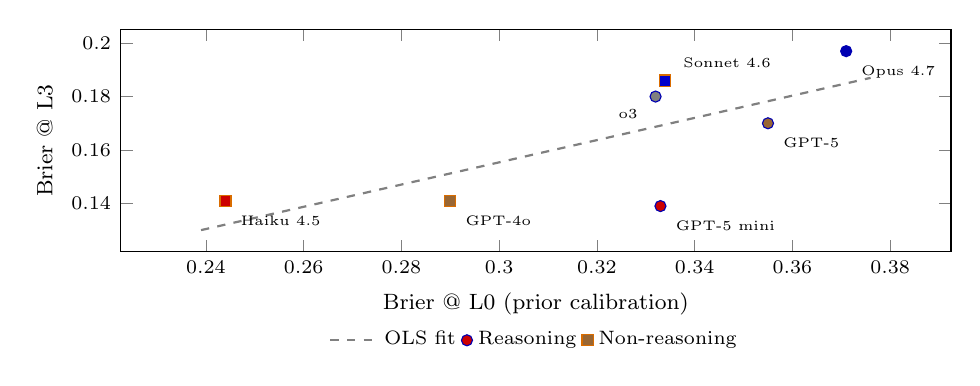
\begin{tikzpicture}
    \begin{axis}[
      width=\columnwidth, height=4.4cm,
      xlabel={Brier @ L0 (prior calibration)},
      ylabel={Brier @ L3},
      enlargelimits=0.12,
      legend style={at={(0.5,-0.32)}, anchor=north, legend columns=3, font=\scriptsize},
    ]
      \addplot+[no marks, dashed, thick, color=black!50] coordinates {\brierLoLthreeFit};
      \addlegendentry{OLS fit}
      \brierLoLthreePlots
      \addlegendimage{reasoningmark}\addlegendentry{Reasoning}
      \addlegendimage{nonreasoningmark}\addlegendentry{Non-reasoning}
    \end{axis}
  \end{tikzpicture}
  \caption{Per-model Brier@L0 vs.\ Brier@L3, with OLS fit overlaid.
    Bootstrap-95\% CI on Pearson $r$:
    [$\BootPriorBrierLo$, $\BootPriorBrierHi$] (point estimate
    $\BootPriorBrierMean$). Prior calibration alone is a strong
    predictor of post-evidence skill, consistent with \cref{prop:bound}.}
  \label{fig:brier-prior}
\end{figure}

The simple slope-vs-Brier@L3 correlation in our panel is
$r = \BootSlopeBrierMean$ with bootstrap 95\% CI
[$\BootSlopeBrierLo$, $\BootSlopeBrierHi$], unidentifiable from
$\nModels$ models. Per-model Brier@L0, in contrast, predicts Brier@L3
with bootstrap CI bounded away from zero
($r = \BootPriorBrierMean$,
CI [$\BootPriorBrierLo$, $\BootPriorBrierHi$];
\cref{fig:brier-prior}). The structural reason is
\cref{prop:bound}: slope is mechanically constrained by
$\sqrt{\mathrm{Brier@L0}}$, with empirical OLS slope on
$\sqrt{\mathrm{Brier@L0}}$ of $\drrCoef$.

\paragraph{Hierarchical confirmatory test.}
The full slope $\beta_{m,q}$ shares the $a_{m,q,3}$ term with Brier@L3
mechanically, so a regression of Brier@L3 on $\beta_{m,q}$ would partly
recover that identity. We therefore use the \emph{L0$\to$L2 sub-slope}
$\beta^{02}_{m,q} = (a_{m,q,2} - a_{m,q,0}) / 2$, which is a function
of $a_0, a_1, a_2$ only and is out-of-sample for $a_3$, in a crossed
mixed-effects model
$\mathrm{Brier@L3}_{m,q} = \alpha + \gamma_1\,\beta^{02}_{m,q} +
\gamma_2\,\mathrm{Brier@L0}_{m,q} + u_m + u_q + \varepsilon$ on
$n{=}\hierNcells$ cells. Without prior control,
$\hat\gamma_1 = \hierNaiveSlopeBeta$ (SE $\hierNaiveSlopeSE$, CI
[$\hierNaiveSlopeLo$, $\hierNaiveSlopeHi$]); after adding
$\mathrm{Brier@L0}$, $\hat\gamma_1 = \hierCtrlSlopeBeta$
(SE $\hierCtrlSlopeSE$, CI [$\hierCtrlSlopeLo$, $\hierCtrlSlopeHi$]).
The coefficient roughly triples in magnitude after the prior is
controlled, which is the prior-confound signature \cref{prop:bound}
predicts: sub-slope is positively coupled with prior miscalibration
(low-prior models have more room to update), so the marginal
coefficient understates the conditional updating-skill effect.

\subsection{Dose-response residual ranks models on updating skill}

\begin{table}[t]
  \centering
  \footnotesize
  \setlength{\tabcolsep}{4pt}
  \begin{tabular}{lcccc}
    \toprule
    Model & R? & Br@L3 & $\bar\beta_m$ & $\mathrm{DRR}^{\mathrm{Res}}_m$ \\
    \midrule
    \leaderboardRows
    \bottomrule
  \end{tabular}
  \caption{Per-model leaderboard, sorted by $\mathrm{DRR}^{\mathrm{Res}}_m$.
    Raw slope $\bar\beta_m$ rank correlates with Brier@L3 only at
    Kendall $\tau = \rankTauBrierlThreeVsslope$ (n.s.);
    $\mathrm{DRR}_m^{\mathrm{Res}}$ at $\tau =
    \rankTauBrierlThreeVsdrrres$ ($p < 0.05$) while flipping three
    pairs against raw Brier@L3.}
  \label{tab:drr}
\end{table}

\Cref{tab:drr} reports $\mathrm{DRR}^{\mathrm{Res}}$ alongside raw
slope. With $\nModels$ models the implied ordering is exploratory; the
point of \cref{tab:drr} is the methodology, not a confirmatory
ranking. $\mathrm{DRR}^{\mathrm{Res}}$ is the right axis to report
alongside (or instead of) raw slope when comparing LLM forecasters on
dose-response benchmarks. Note that the top and bottom of the
$\mathrm{DRR}^{\mathrm{Res}}$ ranking both include reasoning and
non-reasoning models, further arguing against treating naive slope as
a paradigm-level fingerprint.

\subsection{LLMs capture $\sim$40\% of the human-crowd update}

We anchor LLM updates against the Manifold human-crowd update on the
same questions. The aggregate panel mean rises from $\dosesAggLZero$ at
L0 to $\dosesAggLThree$ at L3. Both ratios agree: $R_{\text{total}}$ median
$\manifoldTotalMedian$ (CI [$\manifoldTotalLo$, $\manifoldTotalHi$],
$\manifoldTotalN$ pairs) and $R_{\text{marginal}}$ median
$\manifoldMargMedian$ (CI [$\manifoldMargLo$, $\manifoldMargHi$],
$\manifoldMargN$ pairs). The interpretations differ:
$R_{\text{total}}$ measures the fraction of the human-crowd update
the LLM reproduces, while $R_{\text{marginal}}$ measures the fraction
of the gap between the LLM's own prior and the human posterior that
the ladder closes. \textbf{Both come in at $\sim$$\manifoldMargPct$\%,
well below 1.0.} The agreement removes the concern that one ratio is
inflated by LLM prior knowledge that uninformed traders lack; the LLM
does not match the human-crowd response on evidence on either
metric.

\begin{figure}[t]
  \centering
  \begin{tikzpicture}
    \begin{axis}[
      width=\columnwidth, height=4.4cm,
      ybar=1pt, bar width=6pt,
      ymin=0, ymax=1.0,
      ylabel={Capture ratio},
      symbolic x coords={5-mini,4o,Opus,Sonnet,Haiku,GPT-5,o3},
      xtick=data,
      x tick label style={font=\tiny},
      enlarge x limits=0.08,
      legend style={at={(0.5,-0.18)}, anchor=north, legend columns=2, font=\scriptsize},
    ]
      \addplot+[fill=blue!50!black, draw=blue!70!black] coordinates {\captureTotalCoords};
      \addlegendentry{$R_{\text{total}}$}
      \addplot+[fill=orange!70!black, draw=orange!85!black] coordinates {\captureMargCoords};
      \addlegendentry{$R_{\text{marginal}}$}
      \draw[dashed, red, thin] (axis cs:5-mini,1) -- (axis cs:o3,1);
      \node[font=\tiny, red] at (axis cs:o3,1) [anchor=south east, yshift=1pt] {matches human};
    \end{axis}
  \end{tikzpicture}
  \caption{Per-model median Manifold capture ratios. Dashed red line:
    ratio of 1.0 (LLM update matches human-crowd update). The two
    metrics agree directionally; the apples-to-apples concern that
    $R_{\text{total}}$ conflates better LLM priors with conservative
    updating is not borne out.}
  \label{fig:capture}
\end{figure}

Per-model capture ratios (\cref{fig:capture}) range from 0.20
(Opus~4.7) to 0.92 (GPT-5~mini) on $R_{\text{total}}$, and
0.23 to 0.62 on $R_{\text{marginal}}$. Only GPT-5~mini exceeds 0.6
on the marginal ratio, the cleaner conservatism measure; six of
seven models cluster below 0.5.

\subsection{Question identity explains $\creFracQuestionPct$\% of variance}

A crossed random-effects model
$\mathrm{Brier@L3}_{m,q} = \mu + u_q + v_m + \varepsilon_{m,q}$
fit on the $\nModels \times \nQuestions$ cells yields
$\hat\sigma^2_q = \creVarQuestion$,
$\hat\sigma^2_m = \creVarModel$,
$\hat\sigma^2_\varepsilon = \creVarResidual$,
for variance shares of $\creFracQuestionPct$\% (question) and
$\creFracModelPct$\% (model). The between-model variance component is
estimable but at the small end of the parameter space; the point
estimate ratio is $\creRatioQM{:}1$. Leave-one-model-out re-estimation
bounds the question share to [$\looFracQMin$\%, $\looFracQMax$\%]. We
take this as evidence that benchmark design, not model selection, is
the principal lever for the field's measurable progress on
forecasting.

A Murphy decomposition (reliability $-$ resolution $+$ uncertainty,
five equal-width bins) shows that L0 to L3 increases mean resolution by
$\brierResGain$ versus reducing reliability by $\brierRelReduction$
($\Delta_{\text{res}}>|\Delta_{\text{rel}}|$ for six of seven models):
the ladder's effect on skill is primarily through discrimination, not
confidence calibration. We use this to motivate $\mathrm{DRR}^{\mathrm{Res}}_m$
above; the cross-model correlations between L0 and L3 Murphy components
are exploratory at $n{=}\nModels$ and we make no confirmatory claim
from them.

\section{Discussion}

\paragraph{What an honest dose-response evaluation looks like.}
\Cref{prop:bound} forces a redesign: plot $\mathrm{DRR}_m^{\mathrm{Res}}$
rather than $\bar\beta_m$, anchor "how much did the model update" to a
measured human-crowd reference, and stratify Brier by question.

\paragraph{The variance-bottleneck consequence.}
With $\creFracQuestionPct$\% of variance carried by question identity
and the between-model component at the small end of identifiability,
percentage-point differences between models on any AI-forecasting
leaderboard drawn from a different question pool are statistically
indistinguishable from question-mix noise. The implication is not that
all LLM forecasters are equivalent in some deep sense, but that the
\emph{instrument} (a benchmark with a fixed question pool) has lower
discriminating power than the leaderboard reports imply. Benchmarks
should report question-stratified Brier rather than aggregate Brier,
and treat leaderboard movement inside the
$\sigma_{\text{question}}$ band as null until shown otherwise.

\paragraph{Limitations.}
\label{sec:limitations}
First, our panel has $n{=}\nModels$ models and the cross-model
correlations therefore have wide bootstrap CIs; we report point
estimates as exploratory and rely on structural arguments and the
crossed random-effects fit for confirmatory claims. Second, ladders
were generated by Opus~4.7, which is in the elicitation panel;
we provide a same-family ablation in \cref{sec:ablation}. Third, the
question distribution is Manifold-Markets-specific; the prior-confound
result is structural and should replicate, but the specific numerical
magnitudes are sample-dependent.

\section{Conclusion}

Slope is a mechanical function of headroom, and headroom is a
function of prior calibration. The cleaner anchor for "how much did
the LLM update" is a measured human-crowd update on the same
questions; against that anchor, LLMs close roughly
$\manifoldMargPct$\% of the gap between their prior and the human
posterior (CI [$\manifoldMargLo$, $\manifoldMargHi$]). Between-model
variance in raw Brier@L3 is dwarfed by question-mix variance; once
prior calibration is controlled, the prior-controlled updating-skill
component (\textit{DRR}$^{\mathrm{Res}}$) does discriminate models
meaningfully, though within a narrow absolute range. Dose-response
evaluation is useful, but only with prior control, human anchors, and
question stratification.

\bibliography{paper}
\bibliographystyle{icml2026}

\newpage
\appendix
\onecolumn
\section{Reproducibility}
\label{app:reproducibility}

Code and data will be released upon publication.

\section{Ladder Construction Protocol}
\label{app:ladder}

Each ladder is generated at temperature~0 by Opus~4.7 with the
prompt reproduced verbatim in \cref{app:elicit}. We audit a random 10\%
sample of ladders for resolution leakage, defined as a factual statement
that uniquely entails $y_q$. Ladders failing the audit are
reconstructed.

\section{Elicitation Prompt}
\label{app:elicit}

\begin{verbatim}
You are a careful probabilistic forecaster.

QUESTION: {title}
RESOLUTION CRITERIA: {criteria}
CONTEXT:
{context}

Give your forecast as a single
probability that the question
resolves YES.

Reply with exactly one line in this
format and nothing else:

PROBABILITY: 0.XX
\end{verbatim}

\section{Manifold Anchor: Per-Model Capture Ratios}
\label{app:per-model-capture}

\begin{table}[h]
  \centering
  \begin{tabular}{lccc}
    \toprule
    Model & R? & Median $R_{\text{total}}$ & Median $R_{\text{marginal}}$ \\
    \midrule
    \manifoldCaptureTableRows
    \bottomrule
  \end{tabular}
  \caption{Per-model median capture ratios (total and marginal).
    Capture ratios closer to 1 indicate that the LLM internalises a
    larger fraction of the human-crowd update on the same evidence.}
  \label{tab:per-model-capture}
\end{table}

\section{Ladder Same-Family Ablation}
\label{sec:ablation}

To test whether Opus~4.7's per-question slope is artificially
inflated when reading Opus-authored ladders, we regenerate
$\ablationN$ ladders with GPT-5 (a non-Anthropic-family builder) and
re-elicit Opus~4.7 on the new ladders. Per-question Opus slopes are
then compared pair-wise.

Opus's mean per-question slope was $\ablationOpusLadder$ on
Opus-authored ladders versus $\ablationGPTLadder$ on GPT-5-authored
ladders (mean difference $\ablationDiff$; paired $t$-test
$p{=}\ablationTP$, Wilcoxon signed-rank $p{=}\ablationWP$). The point
estimate is in the opposite direction from the contamination
prediction (Opus is marginally \emph{flatter} on its own ladders, not
steeper) and is statistically indistinguishable from zero. We take
this as bounded evidence against same-family contamination at the
ladder-construction stage; a larger ablation with multiple non-panel
builders would be stronger.

\section{Random-Effects Decomposition}
\label{app:variance}

We fit a single crossed random-effects model using
$\mathtt{statsmodels.mixedlm}$ with $\mathtt{vc\_formula}$ providing a
crossed Model component on top of a Question random intercept. The
fit yields
$\hat\sigma^2_q = \creVarQuestion$,
$\hat\sigma^2_m = \creVarModel$,
$\hat\sigma^2_\varepsilon = \creVarResidual$, giving the variance
shares quoted in §5.4. Leave-one-model-out re-estimation yields
question-shares ranging from $\looFracQMin$\% to $\looFracQMax$\%
across the 7 holdouts.

\section{Contamination Check Details}
\label{app:contamination}

Per-question Pearson correlation of mean Brier@L0 with resolution date
was $\contamR$ ($p = \contamP$). On a median-resolution-date split,
the earlier half ($n = \contamNearly$) had mean Brier@L0
$= \contamEarlyBrier$ versus the later half ($n = \contamNlate$)
$= \contamLateBrier$. The simplest memorisation prediction (recent
questions worse-calibrated) is not observed; we make no positive claim
about contamination beyond the absence of this specific signature.

\end{document}
